\documentclass[12pt, a4paper]{article}

\usepackage[czech]{babel}
\usepackage[IL2]{fontenc}
\usepackage[utf8]{inputenc}
\usepackage{lmodern}  % lepší kvalita PDF

\usepackage[a4paper,top=3cm,bottom=3cm,left=3cm,right=3cm,marginparwidth=1.75cm]{geometry}

\usepackage{graphicx}
\usepackage{titling}
\usepackage{enumitem}
\usepackage{caption}
\usepackage{float}
\usepackage{pdfpages}
\usepackage{verbatim}

\usepackage{pkg-custom-commands}
\usepackage{pkg-url}

% údaje na titulní straně
\title{Hledání min}
\def \thesubtitle {Semestrální práce z předmětu KIV/DB2}
\author{Patrik Harag}
\def \theauthoremail {harag@students.zcu.cz}
\def \theauthorid {(A18N0084P)}

\begin{document}

\begin{titlepage}
	\begin{figure}
		
\includegraphics[height=50mm]{img-fav-logo}
	\end{figure}
	
	\centering
	{\large \hspace{1mm} \par} % tady musí být nějaký text jinak nefunguje vertikální odsazení
	\vspace{15ex}
	
	{\scshape\Large \thesubtitle \par}
	\vspace{1.5ex}
	{\huge\bfseries \thetitle \par}
	\vspace{2ex}
	{\Large\itshape \theauthor \par}
	\vspace{2ex}
	{\texttt{\theauthoremail} \par}
	\vspace{1ex}
	{\texttt{\theauthorid} \par}
	
	\vfill

	{\today\par}
\end{titlepage}

\tableofcontents
\newpage

\section{Zadání}
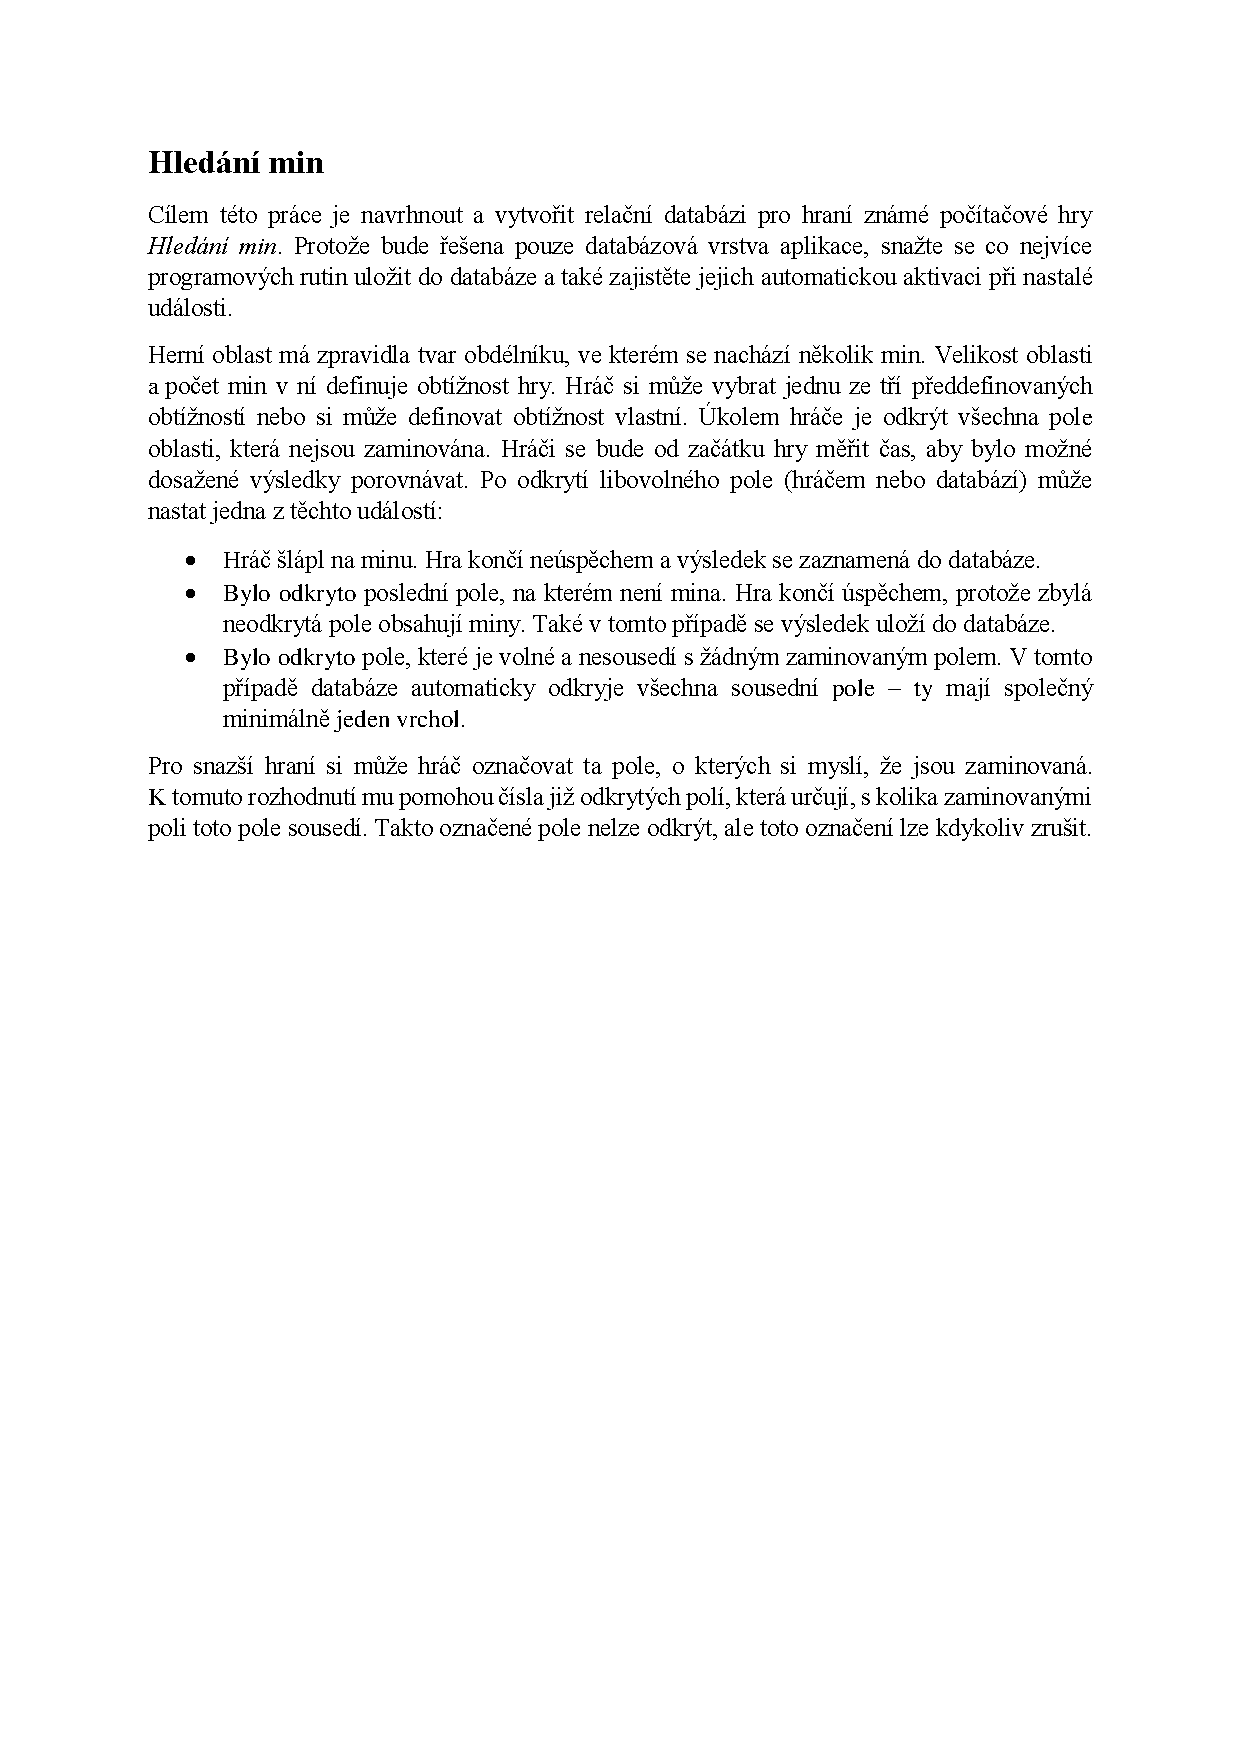
\includegraphics[trim=3cm 800 3cm 100,width=1\linewidth]{assignment}
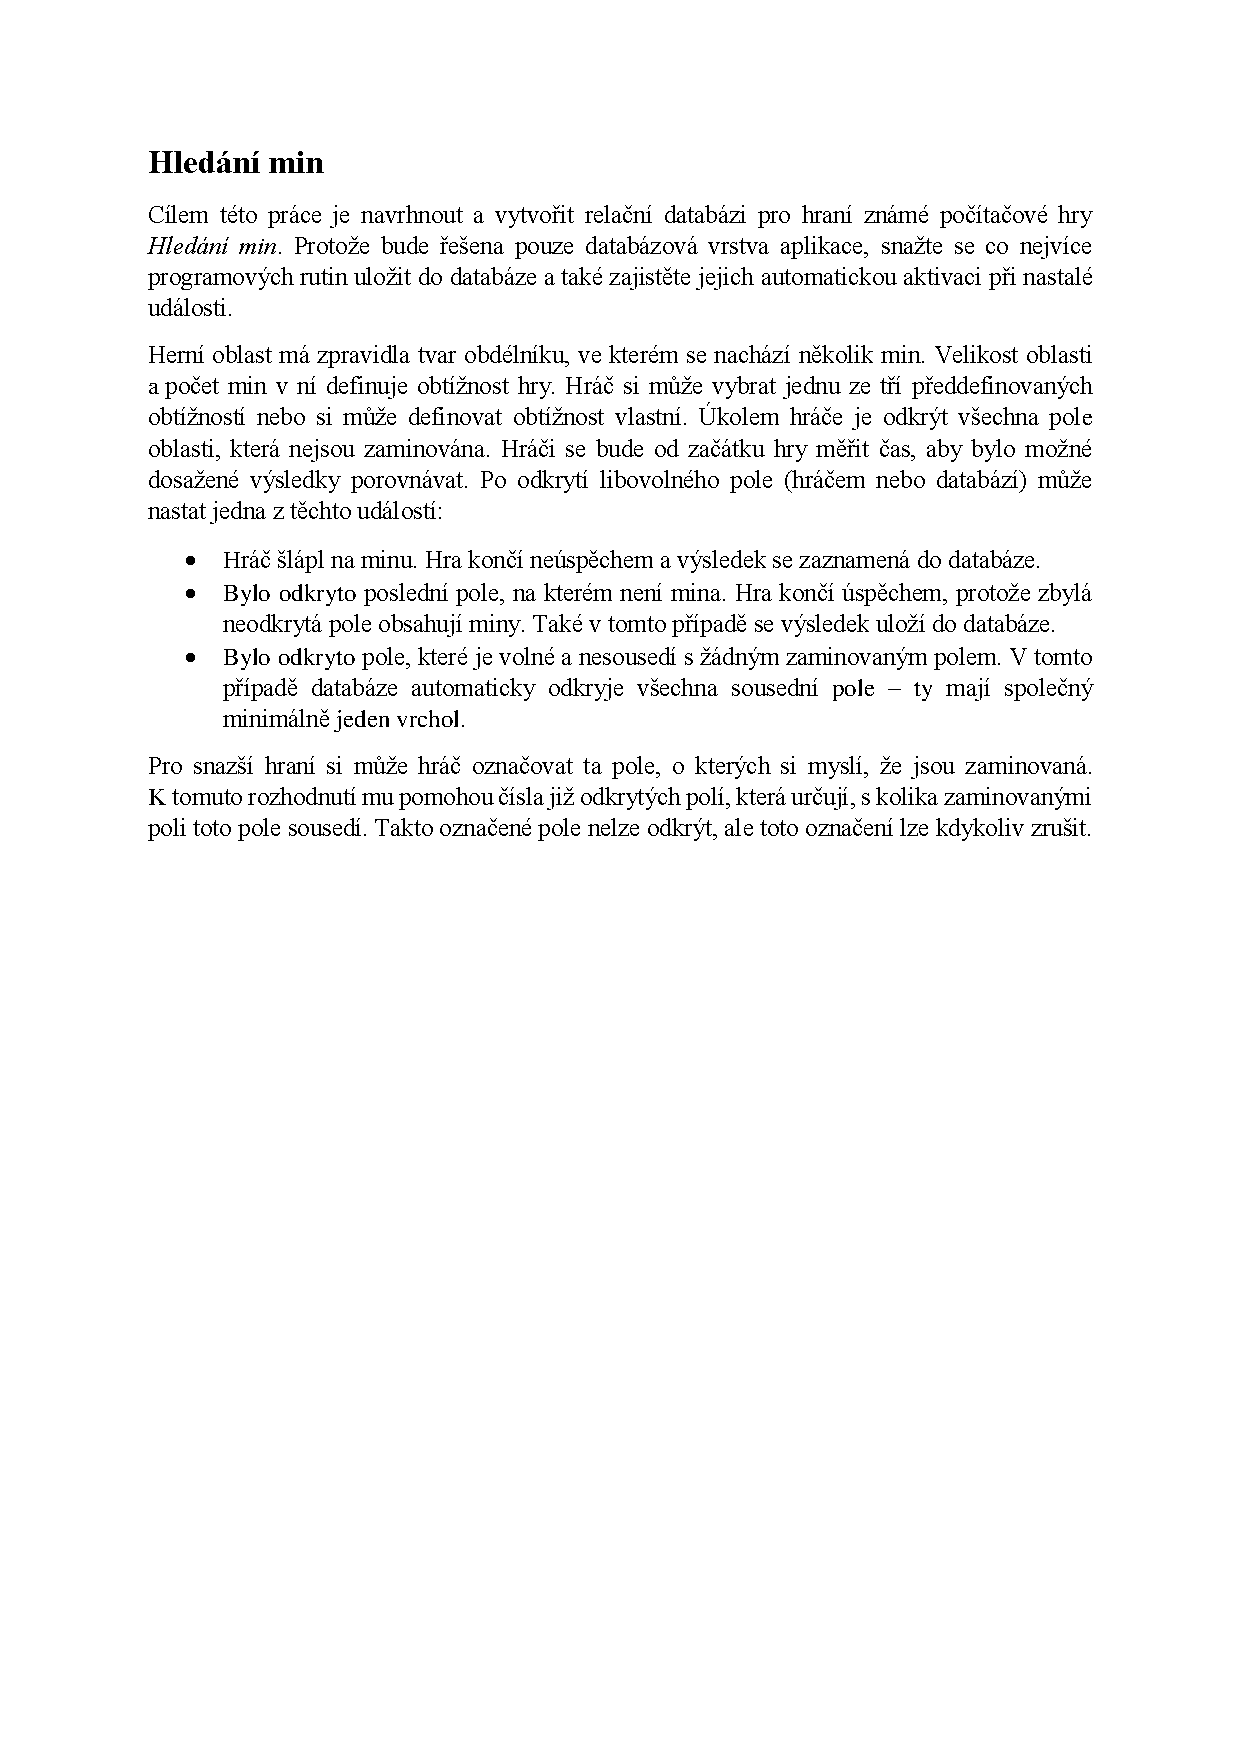
\includepdf[page={2,3,4}]{assignment}

\section{Datová analýza}
Datový model byl vytvořen přesně podle požadavků zadání.
Obsahuje tedy 8 tabulek.
Všechny tabulky až na \emph{OMEZENI} mají definovaný primární klíč – obvykle s~názvem \emph{ID}.
Integrita databáze je zajištěna.
Diagram datového modelu je zobrazen na Obrázku \ref{fig:model}.

\begin{figure}[h]
	\centering
	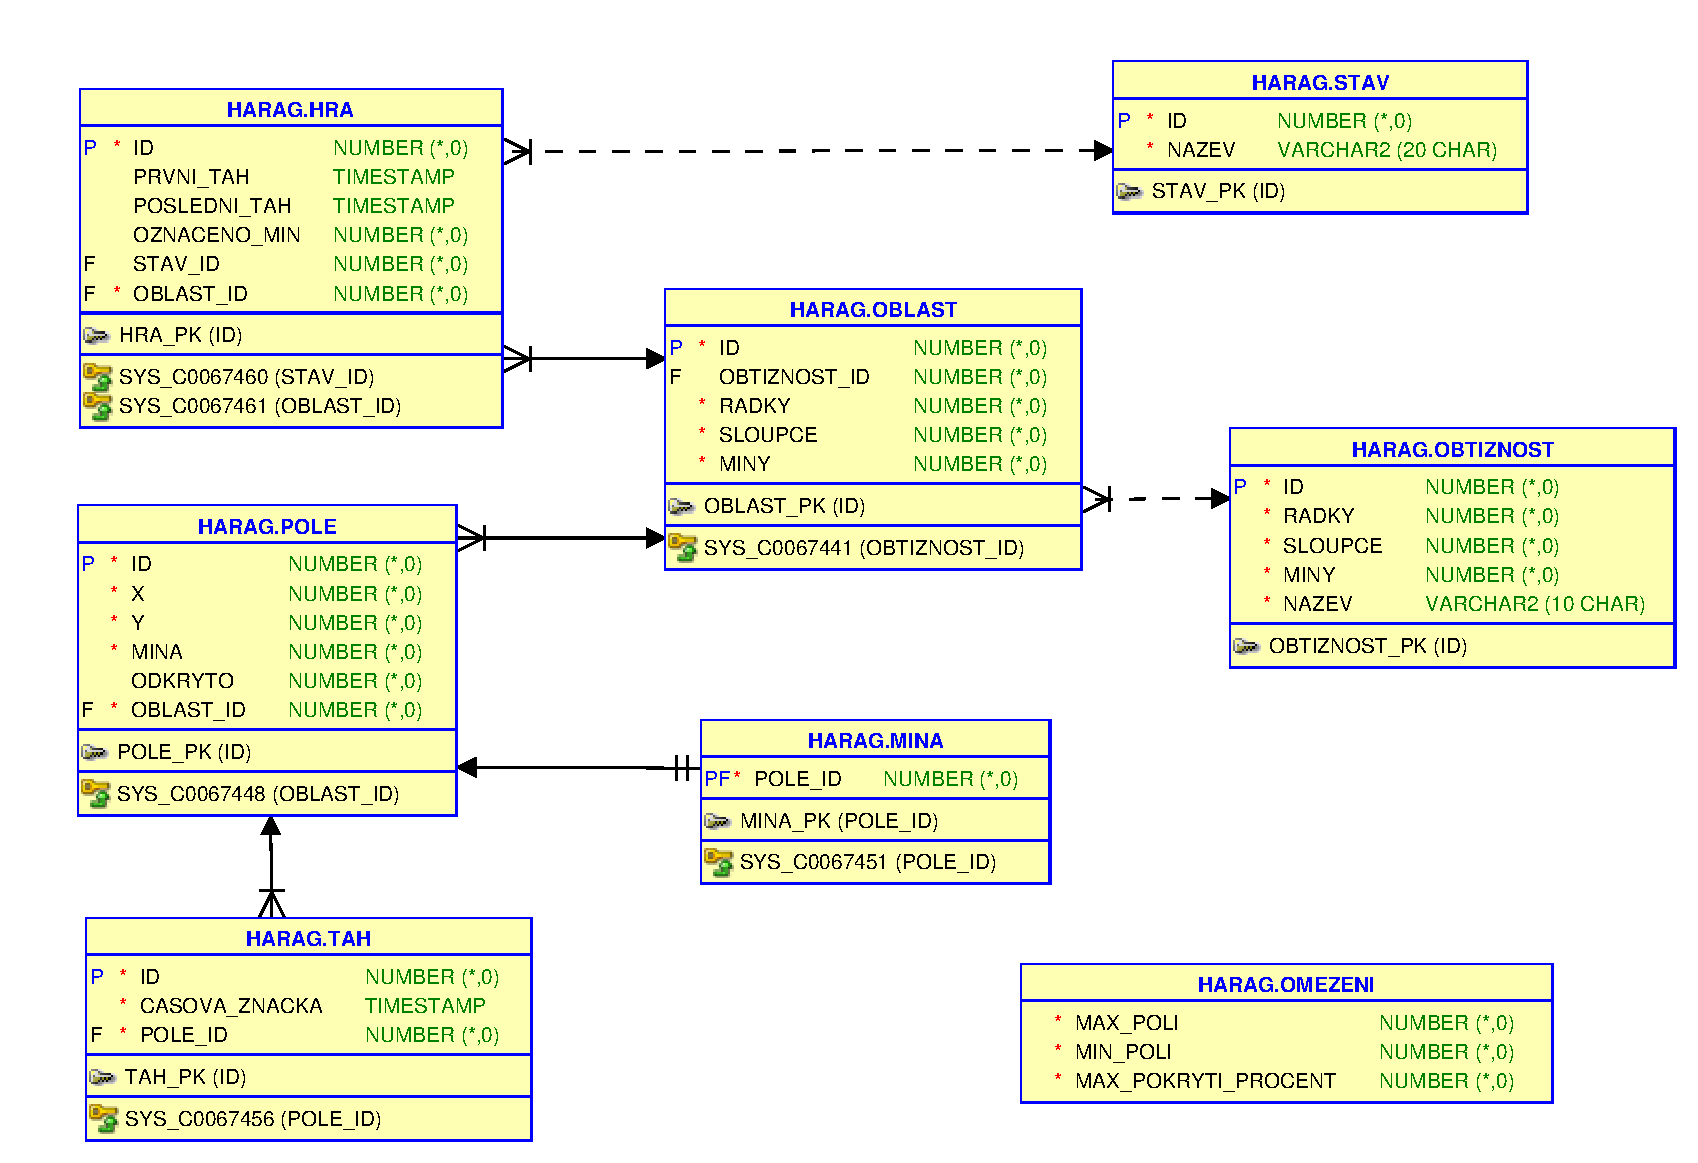
\includegraphics[width=1\linewidth]{model}
	\caption{ER diagram datového modelu}
	\label{fig:model}
\end{figure}

\section{Funkční analýza}
Popis vybrané funkce, procedury, dvou triggerů a dvou pohledů.

\subsection{Trigger T\_OBLAST\_BEFORE\_INSERT}
V případě, že uživatel zvolil předdefinovaou obtížnost, nakopíruje její parametry do tabulky \emph{OBLAST}.
Pokud byly zadány vlastní parametry, dojde k jejich ověření.
Pokud uživatel nezadal ID oblasti, automaticky jej vygeneruje.
\verbatiminput{source-trigger-2.sql}

\subsection{Trigger T\_OBLAST\_AFTER\_INSERT}
Trigger se stará o založení hry, vytvoření polí, zaminování oblasti a vypočtením čísel určujících počet min v okolí, a to po vytvoření nové oblasti.
\verbatiminput{source-trigger-1.sql}

\subsection{Procedura ZAMINUJ\_OBLAST}
Tato procedura slouží k náhodnému zaminování oblasti.
Na vstupu má id oblasti, počet řádků, počet sloupců a počet min.
Její jádro tvoří cyklus. Při každém opakování je náhodně vygenerována pozice.
Pokud na této pozici není mina, dojde k její umístění.
\verbatiminput{source-procedure.sql}

\subsection{Funkce SPATNY\_PARAMETR}
Funkce si načte první řádek z tabulky \emph{OMEZENI} a podle něj zvaliduje parametry hry.
Pokud jeden z parametrů není validní, vrací \emph{TRUE}, jinak \emph{FALSE}.
\verbatiminput{source-function.sql}

\subsection{Pohled VITEZOVE}
Zobrazí všechny hry zakončené vítězstvím včetně trvání hry.
Provádí se napojení na tabulku \emph{OBLAST}, ze které se zobrazují parametry dané oblasti.
\verbatiminput{source-view-1.sql}

\subsection{Pohled PORAZENI}
Podobně jako pohled \emph{VITEZOVE} zobrazí všechny hry zakončené porážkou včetně trvání hry.
Provádí se napojení na tabulku \emph{OBLAST}, ze které se zobrazují parametry dané oblasti.
Navíc obsahuje počet min, které byly správně odhaleny – kvůli tomu obsahuje další vnořený \emph{SELECT}.
\verbatiminput{source-view-2.sql}

\section{Scénář hry}
\subsection{Zahájení hry}
Pro zahájení hry je potřeba nejdříve vložit záznam do tabulky OBLAST.
Je možné využít buď předpřipravené obtížnosti nebo definovat vlastní.
Oba způsoby jsou ukázány níže.
\verbatiminput{source-scenario-1.sql}

\noindent
První vytvořená oblast bude mít ID=0. V dalších ukázkách předpokládejme, že to tak je.

\subsection{Označení miny}
Níže je předvedeno označení miny a zrušení označení.
\verbatiminput{source-scenario-2.sql}

\subsection{Odkrytí políčka}
Níže je předvedeno odkrytí políčka.
\verbatiminput{source-scenario-3.sql}

\subsection{Zobrazení herní plochy}
Níže uvedeným příkazem je možné nechat vypsat herní plochu.
\verbatiminput{source-scenario-4.sql}

\noindent
Význam znaků:
\begin{itemize}
	\item Tečka (.) -- neodkryté políčko,
	\item Číslo (0-8) -- počet min v okolí u odkrytého políčka,
	\item Křížek (\#) -- odkrytá mina (v případě prohry),
	\item Vykřičník (!) -- hráčem označená mina.
\end{itemize}

\subsection{Ostatní}
\verbatiminput{source-scenario-5.sql}

\section{Závěr}
Práce splňuje zadanou funkcionalitu v plné výši.
Navíc byla vytvořena procedura \emph{ODKRYJ\_OBLAST} pro testování hry.

\paragraph{Přílohy}
\begin{itemize}
	\item \code{init.sql} -- script inicializující hru (vytvoří tabulky, triggery, funkce\dots). Po jeho vykonání je možné zahájit scénář hry. V případě opětovného spuštění dojde ke smazání dat a opětovné inicializaci.
	\item \code{test.sql} -- obsahuje vzorové příkazy scénáře hry.
\end{itemize}

\end{document}